
\documentclass[italian,a4paper,10pt]{article}

\usepackage[italian]{babel}
\usepackage{ucs}
\usepackage[utf8x]{inputenc}
%\usepackage[latin1]{inputenc}
\usepackage[T1]{fontenc}
\usepackage{underscore}
\usepackage{graphicx}
\usepackage{subfigure}
\usepackage{wrapfig}
\usepackage{amsmath}
\usepackage{verbatim} 
\usepackage{amssymb}
\usepackage{amsfonts}
\usepackage{listings}
%\usepackage{natbib}
\usepackage[hang,bf,footnotesize,it]{caption}
\usepackage{mdwlist}
\usepackage{boxedminipage}
\usepackage{multirow}


\author{Andrea Rigoni}
\title{Studio del controllo di RFX}
\date{2010-00-00}         

\renewcommand{\theequation}{\thesection.\arabic{equation}}
\newcommand{\vettore}{\overrightarrow}

\newcommand{\deuterio}{D^2_1}
\newcommand{\trizio}{T^3_1}
\newcommand{\elio}[1]{He^#1_2}
\newcommand{\elettrone}{e^+}
\newcommand{\protone}{p^1_1}
\newcommand{\neutrone}{n^1_0}

\newcommand{\Btor}{B_\varphi}
\newcommand{\Bpol}{B_\vartheta}

\newcommand{\tor}[1]{#1_\varphi}
\newcommand{\pol}[1]{#1_\vartheta}
\newcommand{\rad}[1]{#1_r}


\newcommand{\difft}[1]{\frac{\partial #1}{\partial t}}
\newcommand{\diffr}[1]{\frac{\partial #1}{\partial r}}
\newcommand{\diff}[2]{\frac{\partial #2}{\partial #1}}

%\newcommand{\frac1}[1]{\frac{1}{#1}}
\newcommand{\media}{\overline}
\newcommand{\jump}[2]{\left[ #1 \right]_{#2^-}^{#2^+}}

\newcommand{\besKne}[1]{K_m(|n|\epsilon_#1)}
\newcommand{\besKKne}[1]{K'_m(|n|\epsilon_#1)}
\newcommand{\besIne}[1]{I_m(|n|\epsilon_#1)}
\newcommand{\besIIne}[1]{I'_m(|n|\epsilon_#1)}


\newcommand{\mn}{_{m,n}}
\newcommand{\mnp}{_{m',n'}}
\newcommand{\inftyint}{\int_{-\infty}^{+\infty}}
\renewcommand{\imath}{\ensuremath{\dot{\imath}}}




%for CODE listing
\newcommand{\includecodesnip}[1]{\lstinputlisting[stepnumber=0,frame=]{#1}}{}
\newcommand{\includestruct}[1]{\lstinputlisting[stepnumber=0]{#1}}{}
\newcommand{\includecodesample}[1]{\lstinputlisting{#1}}{}

\lstset{
language=Octave,                % choose the language of the code
basicstyle=\footnotesize,       % the size of the fonts that are used
				% for the code
%numbers=left,                   % where to put the line-numbers
%numberstyle=\footnotesize,      % the size of the fonts that are used
				% for the line-numbers
%stepnumber=2,                   % the step between two line-numbers. If
				% it's 1 each line 
                                % will be numbered
%numbersep=5pt,                  % how far the line-numbers are from the
				% code
%backgroundcolor=\color{white},  % choose the background color. You must
				% add \usepackage{color}
%showspaces=false,               % show spaces adding particular
				% underscores
%showstringspaces=false,         % underline spaces within strings
%showtabs=false,                 % show tabs within strings adding
				% particular underscores
				frame=single,                % adds a
				% frame around the code
				tabsize=2,                % sets default
				% tabsize to 2 spaces
%captionpos=b,                   % sets the caption-position to bottom
breaklines=true,                % sets automatic line breaking
breakatwhitespace=false,        % sets if automatic breaks should only
				% happen at whitespace
%title=\lstname,                 % show the filename of files included
				% with \lstinputlisting;
                                % also try caption instead of title
escapeinside={\%*}{*)},         % if you want to add a comment within
				% your code
morekeywords={*,...}            % if you want to add more keywords to
				% the set
}


\begin{document}
\maketitle

\newpage
%capitolo 1
\section{Introduzione}



%\subsection{La ricerca a Padova: l'esperimento RFX}

\subsection{fusione termonucleare}

La fusione termonucleare controllata nasce dall'idea di favorire la
possibilità che due nuclei di atomi leggeri si trovino ad una distanza
inferiore alla barriera columbiana così da permetterne la
trasformazione in unico nucleo di massa superiore. L'avvicinamento
necessario a realizzare questo processo si ottiene per collisione dovuta
ad un'indotta forte agitazione termica (modello classico), a cui
statisticamente si aggiunge un contributo dovuto all'effetto tunnel
(modello quantomeccanico).

Il difetto di massa tra reagenti e prodotti di fusione, e quindi la
quantità di energia liberata, è tanto più marcato quanto maggiore è la
differenza di energia di legame per nucleone rispetto alla variazione di
numero atomico. Ecco perchè risulta vantaggioso utilizzare isotopi di
atomi a basso numero atomico: essi presentano contemporaneamente una
bassa forza columbiana di repulsione, una maggiore energia cinetica
rispetto all'atomo non caricato, è un'alta differenza di energia di
legame. 

Tipicamente le reazioni studiate sono di quattro tipi:


\begin{align}
 \deuterio + \deuterio & \quad \rightarrow \quad  \elio3 + \neutrone + 3.3MeV \\
 \deuterio + \deuterio & \quad \rightarrow \quad  \trizio + \protone + 4.0MeV \\
 \deuterio + \elio3    & \quad \rightarrow \quad  \elio4 + \protone + 18.4MeV \\
 \deuterio + \trizio   & \quad \rightarrow \quad  \elio4 + \neutrone + 17.6MeV
 \label{eq:D-T}
\end{align}

Ognuna possiede una caratteristica sezione d'urto da cui si evince che
la reazione a più alta probabilità è la \eqref{eq:D-T} tra Deuterio e
Trizio\footnote{Trizio prodotto di fissione del Litio ...}. Essa avviene
a valori di energia non inferiori a $5keV$ e raggiunge il massimo di
efficenza a $15keV$. In questa situazione i reagenti si trovano allo
stato di plasma: un gas completamente ionizzato quasi elettricamente
neutro di dimensioni superiori alla lunghezza di Debye
$\lambda_{De}$. A causa dell'alta temperatura non esiste materiale in
grado di contenere la reazione senza inevitabilmente inquinarla.

Una soluzione a questo problema, studiata da oltre 60 anni, è
rappresentata dalle macchine a confinamento magnetico, in cui il
``contenitore'' del plasma è costituito da un gradiente di campo in una
camera a vuoto generalmente toroidale\footnote{un'altro metodo studiato
è l'ICF in cui il confinamento è ottenuto attraverso l'implosione di un
guscio sferico contenente la miscela D-T che viene compressa da raggi
laser o fasci di ioni ad alta energia}.

In siffatto sistema l'obiettivo è quello di soddisfare il cd ``criterio
di Lawson'', ossia di raggiungere uno stato di funzionamento tale per
cui il tasso di reazione sia sufficiente ad autosostenere l'energia
spesa per mantenere il plasma ignito.  La ricerca di un simile risultato
influenza sicuramente la scelta del modello di studio: ad esempio, si
potrebbe ipotizzare di costruire esperimenti di fusione attraverso
acceleratori di particelle, ma la netta predominanza della sezione
d'urto di ionizzazione rispetto alla fusione porterebbe ad un dispendio
di energia di vari ordini di grandezza maggiore rispetto a quella
ricavabile dalla reazione\footnote{ad esempio per una lastra di trizio
colpita da ioni di deuterio si ha: $\sigma_{ion} \approx 10^7
\sigma_{DT}$ quindi per ottenere i 17MeV della fusione sarebbe
necessario un consumo di $10^7$MeV.}.

La progettazione strutturale di ogni macchina da fusione rispecchia la
disposizione scelta per il campo interno. Sono state proposte molteplici
soluzioni geometriche lineari (come la ``bottiglia magnetica'') e
toroidali; quest'ultime sono apparse da subito topologicamente più
vantaggiose, in quanto il toro rappresenta l'unica superficie compatta
connessa orientabile su cui sia possibile definire un campo vettoriale
continuo senza punti critici\footnote{ovvero: definito un campo
vettoriale sulla superficie, non vi è alcun punto in cui esso si
annulli, caratteristica che permette alle linee di campo di ricombinarsi
su se stesse minimizzando l'energia spesa e massimizzando la stabilità
del plasma.}.

Considerando dei parametri specifici per la perdita di energia, come ad
 esempio perdite di frenamento (bremsstrahlung radiation) o di
 collisione (collisional and turbolent phenomena), si può riassumere
 l'efficenza della macchina attraverso un singolo valore detto ``triplo
 prodotto''\cite{cecco}:

\begin{equation}
 n \tau_E T_i \geq 3 \cdot 10^{21} m^{-3}s \cdot keV
\end{equation}

Contemporaneamente si può dimostrare che la curva di ignizione del
plasma che soddisfa il criterio di Lawson mostra un minimo a $T_i \simeq
20keV$; tale valore è la temperatura che si cerca di ottenere nel
bilancio del triplo prodotto variando densità ($n$) e tempo di
confinamento ($\tau_E$).


Per tutte le istallazioni a confinamento elettromagnetico, le
configurazioni del campo consistono in un inseme di componenti
magnetiche toroidali e poloidali; a seconda delle loro caratteristiche,
si dividono in tre principali categorie:
\begin{itemize}
\item{Tokamak}, in cui sono presenti entrambi i campi, ma con netta
     prevalenza di quello toroidale, che ha sostanzialmente la funzione
     di stabilizzare perturbazioni veloci.
\item{RFP} un elaborazione dello \emph{z-pinch}\footnote{vedi infra pg
     xxx} stabilizzato o \emph{screw-pinch}, in cui la componente
     toroidale è equiparabile a quella poloidale al punto da avere
     valore invertito al bordo (da cui il nome, ``reversed field
     pinch''); a questa condizione è affidato il raggiungimento di uno
     stato quiescente del plasma. Rispetto alla configurazione Tokamak
     la stabilità è più critica, ma l'efficenza del sistema è ampiamente
     superiore.
\item{Stellarator} in cui la geometria del campo è costruita disponendo una
     complessa struttura di bobine che favoriscono l'avvitamento della
     colonna di plasma.
\end{itemize}



\subsection{esperimento RFX e configurazioni RFP}


A Padova la ricerca sulla fusione ha condotto negli anni alla
realizzazione della macchina RFX basata sul modello RFP.  

%%%%%%%%%%%%%%%%%%%%%%%%%%%%%FIGURA%%%%%%%%%%%%%%%%%%%%%%%%%%%%%%%%%%%%%
\begin{figure}[ht]
 \centering
 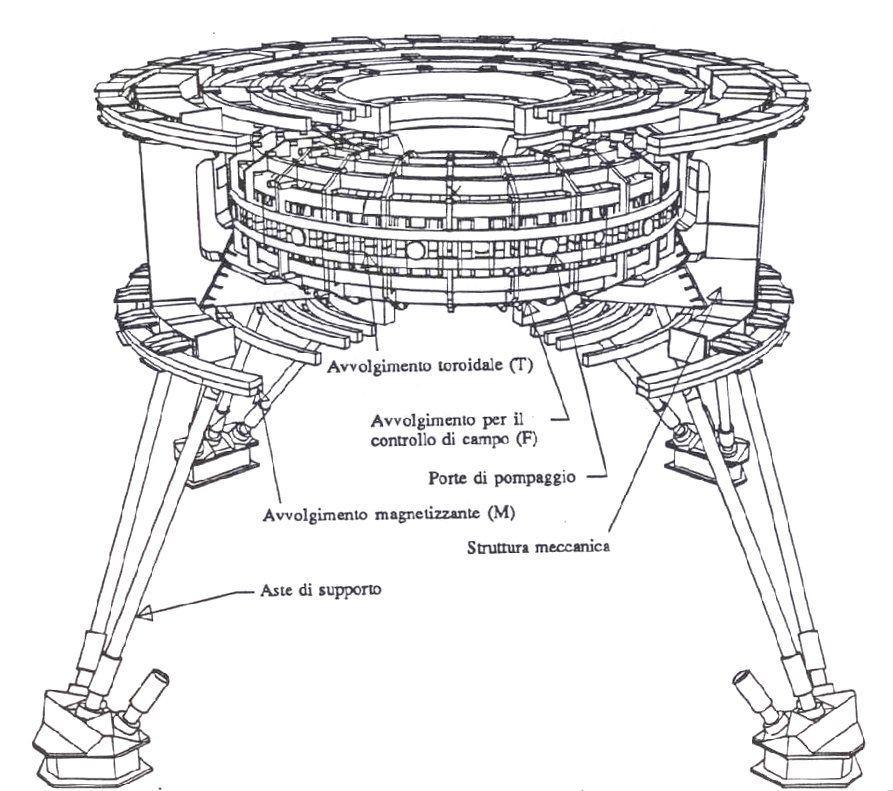
\includegraphics[ width=8cm ] {images/rfx2.jpg}
 \caption{Vista prospettica dell'esperimento RFX}
\end{figure}
%%%%%%%%%%%%%%%%%%%%%%%%%%%%%FIGURA%%%%%%%%%%%%%%%%%%%%%%%%%%%%%%%%%%%%%

La scarica per un sistema \emph{z-pinch} stabilizzato, dove $\Btor \sim
\Bpol$ si origina creando un campo toroidale con le bobine del solenoide
toroidale; attraverso una variazione del flusso concatenato con il toro
si induce poi nel gas una tensione toroidale e quindi, attraverso il
processo di ionizzazione, una corrente $I_p$ che cresce fino a
raggiungere il valore finale voluto. Man mano che la corrente di plasma
sale, si genera un campo poloidale che contribuisce, con la tensione
delle linee e la pressione magnetica, a determinare la situazione di
equilibrio radiale finale. La colonna di plasma quindi viene compressa e
ciò diventa significativo quando i due campi hanno all'incirca la stessa
intensità al bordo: infatti la pressione cinetica del plasma è molto
bassa e la pressione magnetica gioca un ruolo decisivo nella strizione.
Il plasma compresso concentra infatti il campo toroidale e crea nella
zona esterna una regione di quasi vuoto con un plasma tenue a bassa
conducibilità. Si osservano i seguenti profili per $\Btor , \Bpol ,q$.

%%%%%%%%%%%%%%%%%%%%%%%%%%%%%FIGURA%%%%%%%%%%%%%%%%%%%%%%%%%%%%%%%%%%%%%
\begin{figure}[ht]
 \centering
  \subfigure[z-pinch stabilizzato]{ \includegraphics[ width=4cm ]
  {images/profili-zp.png} } 
  \subfigure[reversedfield pinch]{ \includegraphics[ width=4cm ]
  {images/profili-RFP.png} }
  \caption{Profili di $B_\phi$ $B_\theta$ e $q$ rispetto alla posizione dall'asse del toro}
\end{figure}
%%%%%%%%%%%%%%%%%%%%%%%%%%%%%%%%%%%%%%%%%%%%%%%%%%%%%%%%%%%%%%%%%%%%%%

Tale configurazione presenta un minimo nell'andamento del fattore di
sicurezza che comporta uno Shear nullo. Il criterio di Suidam non è
soddisfatto e le superfici adiacenti il punto minimo risuonano
concatenando le linee di campo e innescando una perturbazione instabile.
L'unica soluzione a questo problema è un ribaltamento di $\Btor$ in modo
da rendere monotono l'andamento di $q$:

I primi zeta-pinch stabilizzati entrarono in funzione nei primi anni '60
in particolare il più rilevante fu ZETA con dimensioni simili a quelle
di RFX. I risultati, giudicati sul momento, furono mediocri: la macchina
presentava un regime turbolento, cui talvolta seguiva una fase
quiescente, un fenomeno a quel tempo di difficile spiegazione.

Il primo modello teorico fu proposto da Taylor nel 1974 \cite{taylor}:
egli ipotizzò, e dimostò, che la fase quiescente di ZETA corrispondeva
al passaggio ad una configurazione RFP tramite autorovesciamento del
campo toroidale poiche tale stato doveva corrispondere ad un minimo
energetico.

\begin{comment}
L'imposizione di Taylor fu che, contemporaneamente al minimo energetico,
fosse soddisfatta su tutto il volume di plasma la condizione detta di
``elicità'', ovvero:

\begin{equation}
K_0 = \int_{V_0}\vettore{A} \cdot \vettore{B} dV
\label{eq:elicità}
\end{equation}

mentre l'energia del plasma è considerata trascurando la pressione che
quindi è di natura essenzialmente magnetica:

\begin{equation}
W = \int_V \frac{B^2}{2\mu_0} dV
\end{equation}

La minimizzazione effettuata attraverso moltiplicatore di Lagrange 

\begin{equation}
 \delta(W+ \mu K_0) = 0
\end{equation}

risulta nella relazione:

\begin{equation}
\nabla \times \vettore{B} = \mu \vettore{B}
\label{eq:vincolo_taylor}
\end{equation}

da cui ricordando l'equazione di Maxwell 
$\nabla \times \vettore{B} =\mu_0 \vettore{J}$ 
si ottiene il valore del moltiplicatore:

\begin{equation}
 \mu = \mu_0 \frac{\vettore{J} \cdot \vettore{B} }{B^2} = \mu_0 \frac{J}{B}
\end{equation}

Tale relazione unitamente alla condizione di ``force free equilibrium''
( $\vettore{J}\times\vettore{B} = 0$ ) è stata calcolata nella
approssimazione cilindrica dallo stesso Taylor, e conduce ad una
soluzione dell'andamento di campo descritto tramite funzioni di
Bessel:

\begin{align}
& \Btor = B_0 J_0 (\mu r) \\
& \Bpol = B_0 J_1 (\mu r) \\
& B_r = 0
\end{align}


ricordando il valore di primo zero per la funzione di bessel $J_0$ si
trova che per avere rovesciamento la parete va posta ad una distanza
tale che $\mu a > 2.405$ che confrontato con la \eqref{eq:vincolo_taylor}
porge un valore per il parametro di pinch
\begin{equation}
 \Theta = \frac{\Bpol (a)}{\langle \Btor \rangle} = \frac{\mu a}{2} > \frac{2.405}{2} 
\end{equation}

[finire]
\end{comment}
 







%\section{Il confinamento magnetico di RFX}

\subsection{Le instabilità magnetoidrodinamiche in RFP}
- descrizione magnetoidrodinamica di singolo fluido
- modello magnetostatico
- tipi di instabilità
\newline

Sulla riuscita dei sistemi di contenimento elettromagnetico incidono i
fenomeni di cosidetta instabilità del plasma.

In esperimenti di tipo Tokamak e RFP, le instabilità prodittive di
effetti macroscopici sono descritte, nella loro forma più semplice, dal
modello fluido di plasma MHD (magnetohydrodynamic model). Dato il loro
carattere periodico, queste instabilità sono ben rappresentate da
componenti modali della forma $\exp i(m\theta + n\phi)$, soprattutto in
presenza di un elevato rapporto d'aspetto ed una sezione della camera a
vuoto circolare.

Una volta considerata ogni perturbazione nello spettro delle frequenze spaziali
lungo la colonna di plasma, è con la variazione o la curvatura del campo
che si cerca di riportare il sistema all'equilibrio.
Si noti fin d'ora, tuttavia, che il tentativo di stabilizzazione è vano
se eseguito lungo le superfici magnetiche per le quali i modi
perturbanti risuonano con il passo del fattore di sicurezza pari a
$q=m/n$\cite{wesson}.

\subsubsection{Il modello magnetoidrodinamico}
Tipicamente l'analisi di plasma fluido coinvolge i movimenti
generalizzati di ogni specie ionica, tuttavia è possibile introdurre una
semplificazione condensando in un unico parametro ogni coppia di valori
relativa a ioni ed elettroni, ottenendo un andamento di singolo fluido.
Le grandezze in gioco sono:


\begin{align}
 & \rho_m = n_e m_e + n_i m_i + n_0 m_0 
 && \rho = n_e q_e + n_i q_i
 \\ 
 & \media{J}_m = n_e m_e \media{v}_e + n_i m_i \media{v}_i + n_0 m_0
 \media{v}_0 
 && \media{J} = n_e q_e \media{v}_e + n_i q_i \media{v}_i
 \\
 & \media{v} = \frac{\media{J}_m}{\rho_m} 
 && p \approx n_ekT_e + n_ikT_i
\end{align}

Con queste variabili si possono definire per il fluido le equazioni di
continuità di massa e momento:



\begin{align}
\label{eq:mhd_mass_continuity}
\difft{\rho} + \nabla \cdot (\rho \vettore{v}) &= 0 \\ 
\label{eq:mhd_moment_continuity}
\rho \left(\difft{\vettore{v}} + \vettore{v} \cdot \nabla \vettore{v} \right) &=
\sigma \vettore{E} + \vettore{j} \times \vettore{B} - \nabla p \\
\label{eq:mhd_ohm}
\vettore{E} + \vettore{v} \times \vettore{B} &= \eta \vettore{j} 
%-\frac{ \vettore{j} \times \vettore{B} - \nabla p_e }{ne}
\end{align}

a cui si aggiungono i vincoli di interazione elettromagnetica posti
dalle leggi di Maxwell.
\begin{align}
\nabla \times \vettore{E} &= -\difft{\vettore{B}} \\
\label{eq:ampere}
\nabla \times \vettore{B} &= \mu_0 \vettore{J} \\
\nabla \cdot \vettore{B} &= 0
\end{align}

Il sistema così composto, detto modello \emph{MHD resistivo} del plasma,
risulta non chiuso; sono quindi necessarie ulteriori posizioni
semplificative:

\begin{itemize}
\item si considera la neutralità della carica $\sigma_i \simeq \sigma_e$
      che comporta l'annullamento del termine di resistività $\rho = 0$
      (il plasma è infatti studiato ad una distanza molto superiore alla
      lunghezza di Debye, così da apparire elettricamente neutro);
\item
     si aggiunge un vincolo di stato per il gas ideale, considerando solo
     trasformazioni isoterme o adiabatiche:
     \begin{equation}
     \difft{} \left( \frac{p}{\rho_m^\gamma} \right) = 0
     \end{equation}
     \begin{align}
      & \gamma = 1 && isoterme \\
      & \gamma = 5/3 && adiabatiche
     \end{align}
\end{itemize}

Fatto questo, un primo modo di ottenere una soluzione chiusa del sistema
è inserire l'equazione di Ampere (\ref{eq:ampere}) in quella di
Navier-Stokes della continuità del momento (\ref{eq:ampere}), riducendo
il sistema ad una equazione che descrive il comportamento della
pressione e tensione magnetica del plasma
\begin{equation}
 \label{eq:mhd_sol1}
 -\nabla \left( p+\frac{B^2}{2\mu_0} \right) + \frac{
  (\vettore{B}\cdot\nabla)B}{\mu_0} = 0
\end{equation}
Una seconda soluzione prevede invece l'inserimento dell'equazione di
Ampere in quella di Ohm (\ref{eq:mhd_ohm}), ottenendo la variazione del
campo di induzione che risulta come composizione di un termine di flusso
e un termine di diffusione
\begin{equation}
\label{eq:mhd_sol2}
 \difft{\vettore{B}} = \nabla \times (\vettore{v} \times \vettore{B}) +
  \frac{\eta}{\mu_0} \nabla^2\vettore{B}
\end{equation}

Se consideriamo un esempio semplice di pinch lineare, in cui la
componente di tensione magnetica sia nulla\footnote{la tensione
magnetica è infatti espressione della curvatura delle linee di campo},
si può notare come l'effetto di strizione della (\ref{eq:mhd_sol1})
dipenda dal gradiente di campo della colonna di plasma. Un'importante
figura di merito del confinamento magnetico è, infatti, espressa da
$\beta$, un parametro adimensionale che esprime la pressione cinetica
$p$ rispetto alla pressione magnetica $p_{mag} = B^2/2\mu_0$ e che per
il pinch lineare viene a dipendere proprio dal rapporto tra campo
esterno e campo penetrato:
\begin{equation}
\beta = \frac{p}{p_{mag}} = 1-\frac{B_{int}}{B_{ext}}
\end{equation}

Dal rapporto dei termini di (\ref{eq:mhd_sol2}), considerando come
termine di viscosità $\nu_m=\eta/\mu_0$, si ottiene il \emph{Numero di
Raynolds magnetico} $\mathcal{R}_m$, parametro caratteristico del moto
del fluido:
\begin{equation}
 \frac{\vert \nabla\times\vettore{v}\times\vettore{B}\vert}
  {\vert \nu_m\nabla^2\vettore{B}\vert} \simeq
  \frac{ \frac{v \cdot B}{L} }{ \nu_m \frac{B}{L^2}} = 
  \frac{vL}{\nu_m} \equiv \mathcal{R}_m
\end{equation}

Per ottenere alte pressioni cinetiche è desiderabile avere un plasma con
una ridotta penetrazione e quindi un'esigua viscosità magnetica
($\mathcal{R}_m\gg1$), ma nel contempo, però, si ottiene un moto
turbolento in cui la variazione di campo dipende in misura sempre
maggiore da fenomeni di trasporto.  E' per questo motivo che il modello
di studio per le proprietà di stabilità e per gli effetti della
geometria magnetica sullo stato di equilibio del plasma è ricavato
nell'ipotesi di perfetta conduttività $\eta = 0$ ed è chiamato
\emph{modello MHD ideale}\footnote{Per un'analisi dettagliata delle
condizioni del modello MHD ideale di veda\cite{fridberg}\cite{pizz27}}.

\subsubsection{Equilibrio Statico}
Lo studio dell'instabilità MHD del plasma riguarda principalmente le
perturbazioni del sistema ideale a partire da un punto di equilibrio
magnetostatico. In questo stato le relazioni che presentano una
variazione temporale sono evidentemente nulle, così il sistema,
imponendo $\eta = 0$ e $\difft{}=0$, divene:

\begin{equation}
 \label{mhd_ideal}
 \left\{
  \begin{array}{l}
   \nabla \cdot \vettore{B} = 0 \\
   \nabla \times \vettore{B} = \mu_0 \vettore{J} \\
   -\nabla p + \vettore{J} \times \vettore{B} = 0
  \end{array}
 \right.
\end{equation}
Dalla terza relazione il gradiente di pressione rimane ortogonale alle
linee di campo e corrente, costruendo un insieme di superfici isobare
toroidali\footnote{Si noti che i campi magnetico e di corrente della
prima e seconda relazione sono solenoidali e conducono a superfici
necessariamente chiuse. Se si considera un modulo di pressione costante
lungo detta superficie, con angolo di intersezione tra i vettori di
campo perpendicolare ovunque, si ottiene come soluzione reale possibile
il toro.}, una interna all'altra, chiamate \emph{superfici
magnetiche}\cite{boydsand}.
%\begin{figure}[th]
% \centering
 % \subfigure[gaussiana incorrelata]{images/sup_isabare.jpg}
% \includegraphics[width=5cm , bb= 20 20 575 575]{images/supisobare.jpg} 
%\end{figure}
Queste sono dette \emph{superfici razionali} quando le linee di campo
che le percorrono si ricombinano su se stesse dopo alcuni giri
toroidali, oppure \emph{ergodiche} quando, non ricombinandosi, coprono
l'intera superficie.

Nonostante la struttura fisica toroidale della macchina reale, è
possibile considerare un'approssimazione cilindrica (detta
assialsimmetrica) per semplificare la trattazione delle forze in gioco e
rendere il problema più accessibile, imponendo idealmente di considerare
periodiche anche le grandezze lungo l'asse longitudinale del
cilindro. In questa particolare geometria, che sarà usata anche nel
presente modello di studio, si possono individuare due configurazioni di
corrente che realizzano l'effetto \emph{''pinch''} del plasma
\cite{fridberg}\cite{ortolani} rispettivamente chiamate
$\theta$-\emph{pinch} e $z$-\emph{pinch}, a seconda della direzione
della corrente stessa\footnote{Ovvero lungo la direzione angolare e
assiale del cilindro come rispettive trasformazioni delle coordinate
poloidale e toroidale.}. Ogni configurazione possiede vantaggi e
svantaggi e le soluzioni proposte tendono a trovare il giusto
compromesso nel miscelare le due azioni senza sacrificare la stabilità
che garantisce il tempo di confinamento\cite{boydsand}.  Utilizzando
questo tipo di approssimazione l'equilibrio toroidale è ben descritto
dal modello di Grad-Shafranov tramite un'equazione differenziale
parziale ellittica (GSE) che analizza la stabilità del sistema
(\ref{eq:mhd_ideal}) in termini di funzioni di flusso\cite{boidsand}; la
maggior parte delle configurazioni magnetiche oggi in uso, come i
Tokamak e gli stessi RFP sfruttano questo importante modello di studio.
Introducendo $m$ e $n$ come coordinate poloidale e toroidale del modo
($m,n$) nella trasformazione spaziale in serie di Fourer, possiamo
esprimere l'evoluzione della perturbazione $\tilde{\psi}$ della generica
funzione di flusso analizzata in GSE
\begin{equation}
 \tilde{\psi}(\vettore{r},t) =
  \sum_k{ \tilde{\psi}_k(r) e^{ i(\vettore{k} \cdot \vettore{r} - \omega
  t) } } =
  \sum_k{ \tilde{\psi}_k e^{ i(m\theta + n\varphi - \omega t) } }
\end{equation}
dove $\vettore{r} = (r,\theta,\varphi)$ è il vettore di posizione in
coordinate toroidali e $\vettore{k}$ è il vettore dei relativi numeri
d'onda. La frequenza è invece l'espressione della trasformata nel tempo
ed è in generale un valore complesso $\omega = \omega_R + i\omega_I$,
in cui la parte reale esprime la velocità di propagazione dell'onda e la
parte immaginaria rappresenta la crescita, smorzata $(\omega_I <0)$ o
esponenziale ($\omega_I >0$), dell'ampiezza della perturbazione.  Il passo
di tale perturbazione si ottiene quindi per $(m\theta + n\varphi) =
cost$, ovvero: $$ md\theta -nd\varphi = 0$$ $$ p_p =
\int_0^{\Delta\varphi}d\varphi = \int_0^{2\pi}\frac{m}{n}d\theta =
\frac{m}{n}2\pi$$ Allo stesso modo il passo delle linee di campo
equivale a: $$\frac{Rd\varphi}{rd\theta} = \frac{B_\varphi}{B_\theta}$$
$$p_b(r) = R\Delta\varphi =
\int_0^{2\pi}\frac{1}{R}\frac{B_\varphi(r)}{B_\theta(r)}rd\theta = 2\pi
r\frac{B_\varphi(r)}{B_\theta(r)}$$ La perturbazione $\tilde{\psi}(m,n)$
instabile è, secondo il modello, quella i cui passi sono accoppiati con
le linee di campo; a questo scopo è utile definire il \emph{''fattore di
sicurezza''} $q(r)$ come un unico parametro che rappresenta il valore
dei campi a cui i modi sono accoppiati
\begin{align}
 \label{sec_fact}
  p_b(r) = p_p && \Leftrightarrow &&
 \frac{m}{n} = \frac{r}{R}\frac{B_\varphi(r)}{B_\theta(r)} \equiv q(r) 
\end{align}

A loro volta più superfici adiacenti che presentano uguali fattori di
sicurezza si accoppiano tra loro dando origine a fenomeni di risonanza
secondo il criterio di Suidam (1958) e sono esse stesse fonte di
instabilità; per questo motivo si introduce il parametro detto
\emph{''shear''}
\begin{equation}
 s(r) \equiv \frac{r}{q(r)}\frac{dq(r)}{dr}
\end{equation}
Nella figura [xxx] sono graficati i profili radiali del fattore di
sicurezza per esperimenti Tokamak e RFP; si noti come la configurazione
sia scelta in modo tale da non cadere mai nel valore unitario, e gli
andamenti rappresentino funzioni strettamente monotone.

\subsubsection{classificazione delle instabilità MHD}
Le instabilità sono generalmente classificate in relazione al contesto
fisico considerato; per formulare in modo corretto il problema
magnetoidrodinamico si è visto come sia necessario specificare un insieme
di \emph{condizioni al contorno} che accoppiano il plasma con il campo
magnetico esternamente applicato. Le classi di perturbazioni che si
vogliono analizzare devono quindi rientrare nei vincoli imposti al
sistema per mantenere un significato fisico nell'esperimento reale.

Chiamiamo anzitutto $\tilde{\zeta}(a)=0 $ lo spostamento della colonna
di plasma $\tilde{\zeta}$ e la normale alla superficie non perturbata
$\vettore{n_0}$. Nel caso di \emph{modi interni} (o
\emph{fixed-boundary}) $\vettore{n_0}\cdot\tilde{\zeta}(a) = 0$ non è
necessario uno spostamento del plasma $(\delta W_s = \delta W_v =
0)$. Queste microinstabilità, infatti, non hanno effetti macroscopici
sulla superficie della colonna di plasma, lo degradano soltanto
alterando i coefficienti di trasporto.  I \emph{modi esterni} (o
\emph{free-boundary}) $\vettore{n_0}\cdot\tilde{\zeta}(a)\neq 0$
comportano, invece, lo spostamento dell'interfaccia vuoto-plasma.

Tra questi ultimi, i modi instabili \emph{``pressure driven''},
caratterizzati da numero poloidale $m=0$, sono dovuti a scambi di
flusso, quindi essenzialmente di tipo idrodinamico, e danno luogo ad
instabilità in genere denominate \emph{``interchanges
instabilities''}. Questo tipo di instabilità è facilmente descrivibile
considerando un esperimento z-\emph{pinch} puro in geometria cilindrica;
come visibile in figura [xxx] restringimenti assiali della colonna di
plasma comportano diversi valori di $B_\theta \sim 1/r$; la pressione
cinetica è ovunque la stessa mentre quella magnetica tende ad essere più
forte in corrispondenza della sella, originando rigonfiamenti che
vengono sempre più amplificati.

Una diversa configurazione detta \emph{kink}, illustrata in figura
[xxx], è invece formata da modi $m=1$ cd \emph{''current driven''}. In
questo caso la curvatura della colonna di plasma comporta l'addensarsi
del campo in corrispondenza del raggio di curvatura minore e, quindi, si
assiste anche in questo caso ad un aumento della pressione magnetica che
tende via via ad autoamplificarsi. Rispetto alle instabilità
\emph{pressure driven} le \emph{kink} sono molto pericolose in quanto
rapide e difficilmente controllabili, con tempi di crescita dell'ordine
di $1/\tau_A$\footnote{$\tau_A = a/v_A$, con $v_A$ velocità di Alfvén e
$a$ raggio minore del toro, è riferito a variazioni di campo congelato
al plasma\cite{fridberg} }; esse si formano per la presenza di superfici
risonanti e sono generalmente stabilizzate da un forte campo
toroidale. La condizione di \emph{Kruskal-Safranov}, infatti, impone
$q(a)>1$ come minimo limite per la stabilità delle \emph{kink}, anche se
generalmente per un tokamak si mantiene un rapporto tra campo toroidale
e poloidale tale da avere valori di $q(a)\geq3$. Diverso ovviamente è il
caso di RFP dove la stabilizzazione è un problema più complesso e
coinvolge la presenza di correnti indotte nella scocca della camera
toroidale e, come si dirà a breve, l'uso di controllo attivo.

\subsection{Le instabilità di parete (RWM)}

E' facile notare come in RFP, per mantenere monotono l'andamento del
\emph{fattore di sicurezza}, ovvero \emph{shear} diverso da zero, sia di
fatto necessario il rovesciamento del campo che quindi presenta valore
negativo (e non nullo) in prossimità della parete della scocca. Questa
deve permettere il recircolo della corrente indotta per fungere da
conservatore di flusso; a questo scopo è rivestita da un mantello in
rame che ne aumenta la conduttività.  I \emph{''resistive wall modes''}
(RWM) sono instabilità di tipo \emph{kink} che si formano per la (seppur
esigua) resistenza della parete della camera a vuoto; sono relativamente
lenti poichè dipendono dal tempo di penetrazione del campo nel materiale
del mantello $\gamma_{RWM} \propto 1/\tau_w$.  Questo valore è definito
come:
\begin{equation}
 \tau_w = \mu_0 \sigma r_w \delta_w
\end{equation}
in cui $\sigma$ la conduttività della parete, $r_w$ il suo raggio e
$\delta_w \ll r_w$ il suo spessore. Le RWM sono inoltre caratterizzate
dalla presenza di campo radiale $b_r|_{r=r_s} \neq 0$ (dove $r_s$ è il
raggio relativo alla superficie risonante che genera il modo instabile),
aspetto che rende possibile la ricombinazione delle linee di campo.

La crescita spontanea di instabilità RWM è stata sperimentalmente
osservata in RFP con modi non risonanti $m=1$
\cite{pizz46}\cite{pizz47}\cite{pizz48} e modi
\emph{''pressure-driven''} con $n\neq 1$.  La loro stabilizzazione è
un'importante sfida, poichè esse sono tra i principali fattori che
limitano il raggiungimento di configurazioni ad alto $\beta$ per le
moderne macchine tokamak.

[forse inserire motivo instab TM con effetto RFA]


%\subsection{Il modello di Newcomb - damping rates}
%-


\subsection{L'uso delle saddle coils in RFXmod}

\begin{figure}[ht]
 \centering
 \includegraphics[ width=8cm ] {images/elemento-shell.jpg}
 \caption{sezione della camera toroidale}
\end{figure}

L'esperimento RFX-mod di Padova, come anticipato, consiste in una
macchina a rovesiamento di campo caratterizzata dai seguenti parametri
costruttivi: raggio interno della camera $a=0.459m$, raggio del asse
circolare del toro $R_0 = 1.995m$, corrente massima si scarica
$I\leq2MA$, e durata di aquisizione dell'impulso di $350ms$.  Le
modifiche principali apportate alla precedente versione, operativa nel
periodo 1992-1999, sono state finalizzate al miglioramento del profilo
``sharp-boudary'' del plasma e all'introduzione del controllo attivo dei
modi MHD.  La struttura meccanica della camera a vuoto è costuita in
Iconel 625, mentre all'interno una prima parete di 72x28 piastrelle di
graffite limitano la $Z_{eff}$ delle impurità libere nel plasma e una
seconda parete formata da un guscio (\emph{''shell''}) di rame di 3mm di
spessore ospita le correnti indotte dal campo interno. Il valore di
tempo di penetrazione per un campo verticale si assesta in $t_w = 50
\div 60 ms$ \cite{pizz75}

RFX-mod è equipaggiato con un sofisticato sistema di controllo attivo
composto da 192 bobine a sella (``\emph{saddle coils}'') organizzate in
4x12 array di 4 bobine ciascuno separatamente alimentati e localizzati
sulla superficie esterna della shell alla distanza (media) di $r_c =
0.513m$. I corrispondenti sensori magnetici in grado di rilevare il
campo radiale e toroidale sono posizionati all'interno della parete
conduttiva alla distanza di $r_s = 0.508m$.  Il sistema di amplificatori
è in grado di generare modi non assialsimmetrici m=0 e n < 6 e può
funzionare configurato in diverse modalità: ed esempio lo schema
chiamato \emph{''Virtual Shell''} (VS) è un sistema di retroazione
locale che, pur non tenendo conto degli effetti globali sul plasma, è
già in grado di ridurre fortemente la componente radiale di campo
$b_r$\cite{pizz78}\cite{pizz79}

Il metodo qui presentato aggiunge al precedente la ricostruzione
completa dell'andamento di detta componente, misurata dai 192 sensori,
introducendo un modello per l'attraversamento della parete e l'analisi
delle componenti di aliasing nelle armoniche più elevate.


\newpage
%capitolo 2
\section{Un modello lineare per il controllo dei modi RWM in RFX}

Per collegare l'azione del controllo esterno agli effetti sulla
superficie di plasma mediante metodo magnetoidrodinamico è necessario
conoscere il valore puntuale di campo e del suo differenziale; per
semplificare la trattazione analitica è stato proposto in \cite{pizz81}
un modello di RFP cilindrico lineare\footnote{in appendice è riportata
le formulazione per gli operatori differenziali in coordinate
cilindriche utilizzati nel modello lineare.}. Lo schema considerato
prevede una zona di quasi vuoto che separa la colonna di plasma dalla
parete.  I sensori, coassiali alle bobine di controllo, possono ricavare
misure di campo radiale, poloidale e toroidale, interne ed esterne (in
seguito rispettivamente $b^r,b^{p\pm},b^{t\pm}$).  Sono considerate
evoluzioni temporali esponenziali per le grandezze perturbate, ovvero
caratterizzate da un andamento temporale del tipo $e^{\gamma t}$. Il
modello sfrutta la posizione detta di \emph{thin shell} che considera la
parete della camera a vuoto come un conduttore omogeneo sottile per
ottenere una semplificazione della analisi teoretica.  Lo schema
generale del controllo prevede una composizione in componenti di Fourier
della perturbazione rilevata, di seguito un amplificatore a controllo
digitale genera un segnale di guadagno per riequilibrare i modi
instabili, infine il valore del segnale di controllo e antitrasformato e
applicato direttamente agli amplificatori.  Si vuole quindi trovare un
legame tra l'azione del controllo e l'effetto prodotto in termini di
campo, rivelato dai sensori posti sulla parete della camera,
interponendo un modello fisico che agisca da cuscinetto.  La reazione
del modello fisico prevede una dipendenza spaziale, che comporta un
ampliamento in frequenza dello spettro nella analisi modale, e la
dipendenza temporale, che si esplica nel comportamento della parete alla
penetrazione del campo.

\subsection{Estensione Armonica}

L'applicazione del campo di controllo discretizzato alle posizioni delle
bobine attive, lungo la direzione poloidale e toroidale della camera,
introduce una inevitabile dispersione in frequenza.
Si cerca di trovare un'espressione spettrale completa dell'effetto di
una generica componente armonica nella corrente di controllo $I\mn$.

L'espressione cercata non può prescindere dalla geometria delle bobine
oltre che dalla loro dislocazione.  E' importante ricordare che il
modello dipende da una approssimazione cilindrica di raggio $a$ e
periodicità lungo l'asse $f(r,\vartheta,z) = f(r,\vartheta,z+2\pi
R_0)$. Nel modello sono considerati due strati di bobine: la griglia dei
sensori, capaci di misurare componenti di campo in prossimità della
superficie interna della parete, e la griglia degli attuatori alla
distanza $r_f > r_w$. Le griglie sono formate da serie di $M_c \times
N_c$ solenoidi rispettivamente lungo la direzione poloidale e toroidale.
E' inoltre possibile senza commettere un errore aprezzabile, assumere
che tali solenoidi siano distribuiti ad angolo regolare e presentino
tutti la stessa dimensione.

Come analizzato in \cite{pizz_81} si considera valida la posizione di
\emph{thin shell} che sarà discussa nel prossimo paragrafo, è quindi
possibile esprimere la densità di corrente attraverso una funzione di
flusso.  La corrente negli avvolgimenti di feedback è rappresentata
attraverso una funzione potenziale $J^f$ così che la densità risulti
$\nabla J^f \times \hat{r}$. Si introduce inoltre per il generico
attuatore la funzione di sagoma $f(\vartheta,\varphi)$ che risulta
unitaria allinterno del profilo della bobina e nulla altrove.  La somma
dei contributi presenta evidentemente una dislocazione discreta del
potenziale:
\begin{equation}
 \label{eq:potenziale}
 J^f(\vartheta,\varphi) = I\mn \sum_{j=0}^{M-1} \sum_{k=0}^{N-1}
  e^{ i (m\vartheta_j+n\varphi_k)} f(\vartheta - \vartheta_j,\varphi-\varphi_k)
\end{equation}

dove $\vartheta_j = j2\pi/M$ e $\varphi_k = k2\pi/N$

la trasformata diventa:




\begin{align}
 FT(J^f) &= J^f\mnp = \frac{1}{(2\pi)^2} \iint_{-\infty}^{+\infty} J^f(\vartheta,\varphi)
  e^{-im'\vartheta} e^{-in'\varphi} d\vartheta d\varphi \nonumber \\
 &=\frac{I\mn}{(2\pi)^2}\sum_{j=0}^{M-1} \sum_{k=0}^{N-1}
 \iint_{-\infty}^{+\infty} f(\vartheta - \vartheta_j,\varphi-\varphi_k)
 e^{i(m\vartheta_j+n\varphi_k)} e^{-i(m'\vartheta + n'\varphi)}
 d\vartheta d\varphi  \nonumber
\end{align}
aggiungendo e sottraendo un termine si ottiene:
\begin{align}
 m\vartheta_j - m'\vartheta + m'\vartheta_j - m'\vartheta_j &=
 (m-m')\vartheta_j - m'(\vartheta - \vartheta_j) \nonumber \\
 n\varphi_k - n'\varphi + n'\varphi_k - n'\varphi_k &=
 (n-n')\varphi_k - n'(\varphi - \varphi_k) \nonumber
\end{align}
la funzione diviene:
\begin{align}
 \label{eq:dimostrazione_sideb}
= \frac{I\mn}{(2\pi)^2} \sum_{j=0}^{M-1}\sum_{k=0}^{N-1}
 \iint_{-\infty}^{+\infty} f(\vartheta - \vartheta_j,\varphi-\varphi_k)
 e^{-im'(\vartheta-\vartheta_j)}e^{-in'(\varphi-\varphi_k)}  d\vartheta
 d\varphi \nonumber \\
 \times \quad e^{i(m-m')\vartheta_j}e^{i(n-n')\varphi_k} \nonumber \\
 = I\mn F_{m',n'} \frac1{M} \sum_{j=0}^{M-1} \exp\left(2\pi i
 \frac{m-m'}{M}j \right) \cdot 
 \frac1{N} \sum_{k=0}^{N-1} \exp\left(2\pi i \frac{n-n'}{N}k \right)
\end{align}

dove si sono sostituiti i valori $\vartheta_j = j2\pi/M$ e
$\varphi_k=k2\pi/N$. La funzione di forma trasformata è riassunta in:

\begin{equation}
 F\mn = \frac{MN}{(2\pi)^2}\iint_{-\infty}^{+\infty}
  f(\vartheta,\varphi)e^{-i(m\vartheta+n\varphi)} d\vartheta d\varphi
\end{equation}
In generale per un solenoide di forma rettangolare si assume il valore \cite{pizz81}
\begin{equation}
 \label{eq:shape_coils}
 F\mn = \frac{MN}{\pi^2}\frac{sin(m\Delta\vartheta_f/2)sin(n\Delta\varphi_f/2)}{mn}
\end{equation}

Per concludere, si è precedentemente posto la funzione di forma come
nulla fuori dall'area del solenoide e di valore unitario all'interno,
questo comporta che le somme in (\ref{eq:dimostrazione_sideb}) sono non
nulle per tutti i valori interi di $(m-m')/M$ e $(n-n')/N$; da cui
l'espressione per la generica componente armonica del potenziale:
\begin{equation}
 J\mn^f = F\mn \sum_{l=-\infty}^{+\infty}\sum_{p=-\infty}^{+\infty} I_{m+lM,n+pN}
\end{equation}
Si conclude che ogni modo $(m,n)$ esternamente applicato genera un
numero infinito di armoniche in $J^f$, ognuna delle quali separata da
multipli del numero di bobine del corrispondente asse.

Allo stesso modo anche il sistema di bobine che registrano il campo alla
parete introducono degli artefatti nello spettro, dovuti alla loro
dislocazione discreta. Come già delineato parlando della struttura
geometrica della macchina RFX, sensori e attuatori sono in numero uguale
e coassiali, cosicchè é semplice intuire come le bande laterali che
generano siano per costruzione uguali. Si assume quindi di introdurre
l'effetto di estensione armonica dei sensori con $S\mn$ \cite{pizz_81}
\begin{equation}
 \label{eq:shape_sensori}
 S\mn = \frac{sin(m\Delta\vartheta_s/2)}{m\Delta\vartheta_s/2}
\frac{sin(n\Delta\varphi_s/2)}{n\Delta\varphi_s/2}
\end{equation}
Tale effetto sagoma le componenti del campo che investe i sensori
producendo il profilo del campo rivelato:
\begin{equation}
 B\mn = \sum_l \sum_p S_{m+lM,n+pN} b_{m+lM,n+pN}
\end{equation}

Un metodo alternativo ma ugualmente efficace, per analizzare l'estensione
armonica dei modi introdotti dal controllo, consiste nel considerare la
teoria dei segnali imponendo la disposizione spaziale delle bobine come
la successione dei campioni di un segnale bidimensionale. Una soluzione
tipicamente adottata nell'elaborazione delle immagini.

L'analisi dei segnali è convenientemente studiata attraverso una
\emph{teoria unificata} \cite{cariolaro} dove la generica trasformata
di Fourier presenta sempre nucleo esponenziale ma utilizza la
formulazione di Haar per l'integrazione:
\begin{equation}
 F({\bf v}) = \int_I d{\bf u} f({\bf u})e^{i2\pi{\bf u}^T{\bf v}} \quad \quad
  \begin{array}{r}
   {\bf u} \in I \\
   {\bf v} \in \hat I
  \end{array}
\end{equation}
Il dominio di definizione $I$ e il corrispondente dominio duale $\hat I$
sono costituiti da gruppi regolari genericamente espressi in forma
quoziente: $$ I = \frac{I_0}{S} \longleftrightarrow \hat{I} =
\frac{S^\star}{I_0^\star} $$ dove il gruppo denominatore indica la
periodicità, il numeratore la discretizzazione, e l'opratore $\star$
indica il gruppo reciproco come: $$J^\star = \{{\bf v}| {\bf
u^Tv}\in\mathbb{Z} ,\quad {\bf u}\in J \}$$ Questa digressione puramente
teorica è utile, poichè si può pensare alla distribuzione delle
\emph{saddle coils} come ad un reticolo bidimensionale ortogonale
$\mathbb{Z}(d_1,d_2)$, dove $d_1 = 2\pi/M$ e $d_2 = 2\pi/N$. In questo
modo il segnale di controllo diventa bidimensionale discreto e periodico
di $M\times N$ campioni mentre la trasformata, come integrale di Haar,
diviene la usuale trasformata discreta (DFT) e porge quindi un segnale
definito nel dominio duale con la stessa periodicità e
discretizzazione. Successivamente, si applica una interpolazione del
dominio tramite convoluzione del segnale con la funzione di sagoma
$f(\vartheta,\varphi)$; il dominio di definizione presenta comunque la
stessa periodicità ma diviene una funzione continua. Nel dominio duale
il prodotto di convoluzione è invece un semplice filtraggio che modula
in ampiezza le infinite armoniche eliminandone la periodicità.




\subsection{Matching Procedure}
L' andamento completo del campo, tipico problema di valori al contorno
  \cite{jackson}, è formalmente risolubile mediante equazioni di Green,
  ma tale metodo non sempre risulta agevole
  analiticamente. L'alternativa spesso utilizzata è un approccio che
  parte direttamente dalla formulazione differenziale e usa uno sviluppo
  in funzioni ortogonali.  Nella regione di vuoto tra il plasma e la
  parete ($r<r_w$) e tra la parete e le bobine di controllo
  ($r_w<r<r_f$) vale l'equazione di Poisson, e il campo è quindi
  misurabile attraverso un gradiente di potenziale magnetico:
\begin{align}
 \label{eq:Poisson}
 \nabla^2\Phi = 0 \\
 \label{eq:grad_phi}
 \vettore{b} = \nabla\Phi
\end{align}
Lo sviluppo della (\ref{eq:Poisson}), proposto in appendice, è
realizzato mediante separazione ortogonale delle variabili e nel caso
cilindrico comporta un andamento del potenziale caratterizzato dalla
equazione differenziale di Bessel e di seguito descritto tramite
Funzioni di Bessel modificate (MBF):
\begin{equation}
 \Phi_r = A \cdot I_m(|n|\epsilon_r) + B \cdot K_m(|n|\epsilon_r)
\end{equation}
in cui $\epsilon_r = r/R_0$.

Il campo radiale risultante è ovunque dato come combinazione delle
derivate parziali prime rispetto al raggio $I'_m(|n|\epsilon_r)$ e
$K'_m(|n|\epsilon_r)$. Uno schema del profilo del campo generato dalle
bobine a vuoto è disegnato in figura~\ref{fig:matchb}; si nota
immediatamente un massimo nelle vicinanze del punto di applicazione
della corrente di controllo e via via una attenuazione lungo la sezione
nelle due direzioni opposte.  Si dovranno quindi ricavare i valori dei
coefficienti A e B che realizzino tale profilo. Osservando l'andamento
asintotico delle MBF, graficate per alcuni valori del parametro m in
figura~\ref{fig:bessel}, è immediato rilevare che per l'annullarsi del campo
nelle due direzioni si dovranno eliminare le componenti non
asintoticamente nulle; ovvero porre $B = 0$ per $r<r_w$, successivamente
$A\neq0 ,B\neq0$ nell'intervallo $r\in[r_w,r_f]$, e infine $A=0$ per
$r>r_f$.

%%%%%%%%%%%%%%%%%%%%%%%%%%%%%FIGURA%%%%%%%%%%%%%%%%%%%%%%%%%%%%%%%%%%%%%
\begin{figure}[ht]
 \centering
 \includegraphics[ width=8cm ] {images/matchb.png}
 \caption{Schema del profilo di campo radiale}
\end{figure}
%%%%%%%%%%%%%%%%%%%%%%%%%%%%%FIGURA%%%%%%%%%%%%%%%%%%%%%%%%%%%%%%%%%%%%%

%%%%%%%%%%%%%%%%%%%%%%%%%%%%%FIGURA%%%%%%%%%%%%%%%%%%%%%%%%%%%%%%%%%%%%%
\begin{figure}[ht]
 \centering
 \includegraphics[ width=8cm ] {images/BesselI.png}
 \caption{Schema della funzione MBF I per valori di m=0,m=1,m=2,m=3}
\end{figure}
%%%%%%%%%%%%%%%%%%%%%%%%%%%%%FIGURA%%%%%%%%%%%%%%%%%%%%%%%%%%%%%%%%%%%%%

%%%%%%%%%%%%%%%%%%%%%%%%%%%%%FIGURA%%%%%%%%%%%%%%%%%%%%%%%%%%%%%%%%%%%%%
\begin{figure}[ht]
 \centering
 \includegraphics[ width=8cm ] {images/BesselK.png}
 \caption{Schema della funzione MBF K per valori di m=0,m=1,m=2,m=3}
\end{figure}
%%%%%%%%%%%%%%%%%%%%%%%%%%%%%FIGURA%%%%%%%%%%%%%%%%%%%%%%%%%%%%%%%%%%%%%




\begin{align}
 b_r &= A_1 \cdot I'_m(|n|\epsilon_r) && r < r_w \\
 b_r &= A_2 \cdot I'_m(|n|\epsilon_r) +  B_2 \cdot K'_m(|n|\epsilon_r) &&
 r_w < r < r_f \\
 b_r &= B_3 \cdot K'_m(|n|\epsilon_r) && r > r_f
\end{align}

Per quanto riguarda le condizioni al contorno sulla parete della camera
gli effetti dei modi RWM devono essere posti in relazione alla dinamica
temporale dell'impulso. La parete, infatti, può essere genericamente
associata ad una impedenza resistiva e induttiva con costante di tempo $L/R$.

Per confrontare i fattori di crescita con la risposta della parete si è
scelta la approssimazione \emph{''complete thin shell''}\footnote{
L'accezione ``completa'' si riferisce alla continuità del guscio;
eventuali tagli o buchi nella forma della parete, impedendo il recircolo
delle correnti indotte, modificano la differenza di campo nel salto di
parete riducendo l'attendibilità dell'aprossimazione.} che sottende alla
relazione:
\begin{equation}
 \frac{\delta_w}{r_w} \ll |\gamma|\tau_w \ll \frac{r_w}{\delta_w}
\end{equation} 
Il tempo caratteristico della parete in termini di $L/R$ equivalenti è
invece ricavabile tramite:
\begin{equation}
 \tau_w = \mu_0\sigma_w r_w \delta_w
\end{equation}
con $\delta_w$ spessore e $\sigma_w$ conducibilità del guscio.

In questo modo si assume irrilevante la densità di corrente radiale che
attraversa il sottile spessore $\delta_w$, così che le altre componenti
(e quindi il campo radiale) siano costanti e proporzionali alla
differenza tra campo trasversale interno ed esterno($b^{p\pm},b^{t\pm}$).

Con queste ipotesi possono essere dimostrate \cite{pizz70} le seguenti
relazioni che descrivono il profilo di campo radiale nell'attravesamento
di parete in $r_w$:

\begin{align}
 \label{eq:jump1}
 \jump{b_r}{r_w} &= 0  \\
 \label{eq:jump2}
 \jump{ \diffr{}(rb_r) }{r_w} &= \tau_w \gamma_{m,n}b_r
\end{align}

Nella regione di spazio dove è situato il solenoide attuatore del campo
di controllo si ipotizza un secondo guscio ideale che per il teorema di
equivalenza simula il campo generato attraverso una distribuzione di
correnti impresse sulla superficie. Considerando questo strato
immaginario di spessore $\delta_c$ e interessato dalla corrente
superficiale $\vettore{j} = (\rad{j},\pol{j},\tor{j})$ si identifica un
salto di campo radiale in $\epsilon_c = r_f/R_0$ proporzionale alla corrente
applicata:

\begin{equation}
 \jump{ \diffr{}(\rad{b}) }{r_c} = i \mu_0 \delta_c
  \left( \frac{m^2 + n^2 \epsilon_c^2}{m} \right) j_\varphi
\end{equation}

La densità superficiale $j_\varphi$ è direttamente dipendente dalla
corrente circolante nel solenoide attraverso un parametro geometrico
$\Sigma$:

\begin{equation}
 I_c = 2 \pi r_c \delta_c \Sigma j_\varphi
\end{equation}
Da cui la formula di interesse nel presente lavoro per $m=1$
\begin{equation}
 \label{eq:jump_coil}
 \jump{ \diffr{}(\rad{b}) }{r_f} = i \frac{\mu_0}{2\pi r_f^2 \Sigma}
  \left( {1 + n^2 \epsilon_c^2} \right) I_c
\end{equation}

L'andamento radiale atteso è schematizzato completamente in figura
[figura]: le relazioni al contorno (\ref{eq:jump1}), (\ref{eq:jump2}) e
(\ref{eq:jump_coil}) caratterizzano la continuità della funzione e la
derivata nei punti di giunzione dei tre intervalli. La procedura di
matching consiste allora nel determinare i paramentri $A_1,A_2,B_2,B_3$ per
ottenere un valore di campo $b_r$ lungo il profilo a fronte della
applicazione di una corrente $I_c$; questo valore sarà calcolato nel
campo a vuoto e utilizzato per dimensionare l'effetto del controllo
attivo sul campo disperso dalla parete.

%%%%%%%%%%%%%%%%%%%[figura]%%%%%%%%%%%%%%%%%%%%%%%%%%%%%%%%%%%%%
\begin{figure}[ht]
\caption{profilo del valore di potenziale per valori crescenti della
 coordinata radiale}
\end{figure}

Il campo generato dalla corrente nelle coils e dato da:

\begin{equation}
 \label{eq:bf_coils}
 b^f\mn = -\frac{\mu_0}{R} n^2 \epsilon_f \besKKne{f} \besIIne{f} J^f\mn
  \equiv \frac{\mu_0}{\pi a}c\mn J^f\mn
\end{equation}
[spiegare il termine $\mu_0/\pi a$]
Con $J^f\mn$ si è precedentemente definito il potenziale della
distribuzione delle correnti di modo $m,n$ localizzate sulla superficie
immaginaria in $r_f$ dove:
\begin{equation}
 c\mn = -\pi n^2 \epsilon_a \epsilon_f \besKKne{f} \besIIne{f}
\end{equation}

A questo punto, determinato il campo impresso dalle sorgenti, si ottiene
il valore nel punto di matching attraverso la seguente relazione che
riassume tutta la procedura.

\begin{equation}
 \label{eq:bw_coils}
 \{b^r\mn,b^{p\pm}\mn, b^{t\pm}\mn \}_{sens} =
  \{1,a^{p\pm}\mn,a^{t\pm}\mn\} M\mn b^f\mn
\end{equation}

Il valore $M\mn$ è un coefficiente di mutua induttanza per la relativa
frequenza spettrale, esso è ricavato risolvendo il problema
elettrostatico tramite le sopraindicarte condizioni al contorno. Una
dimostrazione rigorosa per la soluzione seguente è proposta in
appendice:

\begin{equation}
 \label{eq:emme}
  M\mn = - \frac{1}{2\tau_w(s-\gamma\mn)} \frac{1+m^2/n^2\epsilon_w^2}{\besKKne{w}\besIIne{f}}
\end{equation}

con uniformità di simboli si è espressa con $\gamma\mn$ il tasso di
crescita del modo $(m,n)$ analizzato. Si nota immediatamente che la
funzione $M\mn(s)$ presenta un polo corrispondente al tasso di
crescita del RWM corrispondente $s=\gamma\mn$.

I simboli $a^{p\pm},a^{t\pm}$ rendono il rapporto interno ed esterno di
campo poloidale e toroidale rispetto al valore radiale calcolato, ed
equivalgono a:

\begin{align}
 a^{\{p^-,t^-\}}\mn &= s_0\{m,n\epsilon_w\}\frac{d\mn - 1 +
 2\tau_w\gamma\mn}{m^2+n^2\epsilon^2_w} \\
 a^{\{p^+,t^+\}}\mn &= s_0\{m,n\epsilon_w\}\frac{d\mn - 1 +
  2\tau_w(\gamma\mn -s)}{m^2+n^2\epsilon^2_w} 
\end{align}
dove $s_0 = \pm1$ è un termine di segno introdotto per eliminare il
termine immaginario nel campo poloidale, si esegue infatti uno shift di
fase di 90° nel segnale. E' sufficiente porre tale valore a $sign(m)$
oppure $sign(n)$ rispettivamente per i sensori poloidali e toroidali.

Il termine
\begin{equation}
 d\mn = 1 - \left( 1+\frac{m^2}{n^2\epsilon^2_w} \right) \frac{|n|\epsilon_w\besKne{w}}{\besKKne{w}}
\end{equation}
equivale a $rb'_r/b_r$ per il campo magnetico esterno $(r > r_w)$ in
assenza della corrente di feedback applicata.





\subsection{Controllo}


Si può quindi ricostruire una relazione conclusiva che tenga conto di
tutti i passaggi fino ad ora analizzati. Caratterizzando la relazione
iniziale (\ref{eq:bf_coils}) con il termine $J^f\mn$, che tiene conto della
generazione delle \emph{sidebands} e del fattore di forma $F\mn$ di
(\ref{eq:shape_coils}), si ottiene il valore del campo generato dalle
\emph{saddle coils}. Valutando opportunamente il problema elettrostatico
in geometria cilindrica e imponendo le condizioni al contorno della
approssimazione di \emph{thin shell} si ottiene il valore dello stesso
campo (\ref{eq:bw_coils}) attraverso un termine di mutua induttanza
$M\mn$. Infine si aggiunge il contributo spettrale $S\mn$ di
(\ref{eq:shape_sensori}), il termine dovuto ai sensori.  Componendo
tutti i termini si perviene ad una relazione di ingresso/uscita tra la
corrente di controllo e il segnale di campo ricostruito dai sensori per
il feedback. Per ogni modo $(m,n)$ eccitato dal controllo, con $|m|<M/2$
e $|n|<N/2$, si ottiene:

\begin{equation}
 B\mn = \sum_{m'=m+lM}\sum_{n'=n+pN} F\mnp S\mnp M\mnp
  \{1,a^{p\pm}\mnp,a^{t\pm}\mnp\} \frac{\mu_0}{\pi a} I\mnp
\end{equation}
e si considera quindi la funzione di trasferimento del sistema per la
singola componente $(m,n)$
\begin{equation}
 {P_1}\mn = \sum_{\mnp}\frac{\pi a B\mnp}{\mu_0 I\mnp}
\end{equation}
Ciò che si vuole ottenere è un valore di guadagno applicato alle bobine
che annulli il campo rilevato; questo si traduce un un regolatore a zero
caratterizzato dalla seguente funzione caratteristica nella trasformata
di Laplace dove si è indicato con $G\mn(s)$ lo spettro di una generica
funzione guadagno.
\begin{equation}
 1+G\mn(s){P_1}\mn(s) = 0
\end{equation}
[figura]

Ci limitiamo in questo caso a non analizzare sistemi di controllo ottimo
e valutare il solo caso di controllo proporzionale con G indipendente
dal tempo.
Il sistema di figura può essere facilmente rappresentato da un sistema
di stato.
\begin{equation}
 \left\{
  \begin{array}{l}
   \dot{x}(t) = Ax(t) + Bu(t) \\
   y(t) = Cx(t)
  \end{array}
 \right.
\end{equation}
Considerando la reazione statica dall'uscita, si dimostra facilmente che
il sistema può essere ricondotto ad una tipica retroazione dallo stato;
infatti dalla legge di controllo del tipo:
\begin{equation}
 v(t) = Gy(t) + u(t)
\end{equation}
si ricava facilmente 
\begin{equation}
v(t) = GCx(t) + u(t)
\end{equation} ovvero un caso particolare di retroazione dallo stato.

%Si può ulteriormente caratterizzare il polinomio $P1$ per il caso di
%specie. Volendo analizzare modi $m=1$ lo studio può essere eseguito con
%l'ausilio del solo campo radiale. I valori di campo e corrente si
%riducono al caso $(m=1,n)$.

 E' possibile inoltre semplificare la trattazione, condensando i termini
di forma $F\mn$ e $S\mn$ all'interno della mutua induttanza, e definendo
convenientemente un nuovo paramentro che riassume l'intero termine
residuo $R\mn$ \cite{gregoratto} della funzione di trasferimento:
\begin{equation}
 {P_1}\mn = \sum_{m',n'} \frac{R\mnp}{(s-\gamma\mnp)}
\end{equation}
Tutti i poli con tassi di crescita negativi sono instabili e devono
essere controllati.  La somma in $m' = m+lM, n'= n+pN$ ha evidentemente
infiniti termini ma fortunatamente il fattore di forma, come si è
precedentemente mostrato, agisce come un attenuatore per le armoniche
elevate.  Nel contempo sappiamo che anche il plasma si mostra via via
più stabile per modi elevati; é quindi logico pensare di limitare il
numero di addendi alle prime armoniche identificando quali siano i poli
instabili.  Nel procedimento qui adottato, dopo aver ordinato le coppie
zero-polo rispetto alla stabilità del polo, si applica un ulteriore
troncamento del numero di poli per ottenere una utile riduzione della
dimensione del sistema a cui applicare il guadagno.
\begin{align}
 \label{eq:trasferimento}
 {P_1}\mn &= \sum_{j,k} \frac{R\mnp}{s-\gamma\mnp} =
 \frac{b_0+b_1s+\hdots+b_{n-1}s^{n-1}}{a_0+a_1s+\hdots+s^n}
\end{align}
La teoria della realizzazione asserisce che una funzione matriciale
strettamente propria ha sempre soluzione in un sistema in forma canonica
di controllo e una in forma canonica di osservazione.  Volendo indagare
una sigola coppia di modi $(m,n)$ è altresì facilmente dimostrabile che
il sistema in forma canonica di controllo, con le matrici
\newcommand{\canonicalcontrolA}{ 
\left[
\begin{matrix}
 0 & 1 && \\
 &&\ddots \\ \\
 &&&1 \\
 -a_0 & -a_1 & \hdots & -a_{n-1}
\end{matrix}
\right]
}
\newcommand{\canonicalcontrolB}{ 
\left[
\begin{matrix}
0\\ 0\\ \vdots \\ \\ 1
\end{matrix}
\right]
}
\newcommand{\canonicalcontrolC}{ 
\left[
\begin{matrix}
B_0& b_1& \hdots & & b_{n-1}
\end{matrix}
\right]
}
\begin{align}
 A &= \canonicalcontrolA,\quad B = \canonicalcontrolB \\ \nonumber
 \\ C &= \canonicalcontrolC \nonumber
\end{align}
realizza la (\ref{eq:trasferimento}). Infatti si ottiene immediatamente
la funzione di trasferimento con $y(t)/u(t) = C(sI-A)^{-1}B$. Avendo
scelto la realizzazione di una singola coppia $(m,n)$ è anche possibile
dire che essendo i poli tutti separati tra loro numeratore e
denominatore della (\ref{eq:trasferimento}) sono primi tra loro e la
realizzazione è minima. In questo caso gli autovalori della matrice di
stato coincidono con i poli della funzione di trasferimento e sono tutti
allocabili.

%Si considera il tasso di crescita della camera a vuoto con il valore
%definito da C.~G.~Gimblett in \cite{pizz_96} utilizzato nei precedenti
%articoli di R.~Fitzpatrick \cite{pizz_70} e R.~Paccagnella e P.~Zanca
%\cite{pizz_97}.

\newpage
%capitolo 3
\section{Implementazione del modello}

\subsection{Sistema orientato agli oggetti}
Il raggiungimento dell'obiettivo comune e l'enorme quantità di fondi
necessari agli esperimenti pongono la ricerca sulla fusione
termonucleare controllata nel panorama scientifico come uno dei più
vasti ambiti di cooperazione internazionale.  I recenti esperimenti JET
e ITER sono infatti frutto dello sforzo congiunto di molti paesi
consorziati e rappresentano un chiaro esempio di come il lavoro
combinato possa dare una forte accelerazione verso la concretizzazione
dei risultati; dal punto di vista economico agevolati dalla divisione
delle spese e dal punto di vista scientifico arricchiti per la
possibilità di attingere ad esperienze specilistiche maturate nel tempo
dagli stati membri. Per questa ragione è auspicabile se non necessario
orientare lo sforzo di ricerca verso un sistema integrato e standardizzato.

Il modello di studio presentato nel precedente capitolo ha avuto
precedenti implementazioni in riferimento a diversi studi svolti sugli
esperimenti EXTRAP T2R \cite{gregoratto} e RFXmod stesso
\cite{pizzimenti}. Il codice numerico usato nei lavori citati è stato
quì adattato al funzionamento in un ambiente orientato agli oggetti e
riformulato per funzionare in una piattaforma a sorgente aperto.

La programmazione orientata agli oggetti (Object Oriented Programming) è
in generale un paradigma di programmazione, che prevede la definizione
di oggetti software dotati di attributi (dati), e metodi (procedure);
interagenti tra loro mediante scambio di messaggi. Tale scelta, vista
come un supporto alla modellazione software per l'oggetto di studio, è
volta ad ottenere un effettivo supporto naturale alla modularizzazione e
al riuso del codice. La modularità del codice garantisce una maggiore
chiarezza di lettura creando le basi per una piattaforma comune in cui
risulti uniformato l'approccio alle entità di studio.  Di fondamentale
importanza per capire il valore della programmazione ad oggetti é il
concetto di astrazione che storicamente ha visto via via un sempre
maggior sviluppo nel lessico informatico. Un concetto sviluppatosi
inizialmente all'interno della così detta programmazione procedurale che
per prima propose l'idea di interfaccia per nascondere i dettagli
dell'implementazione e la connessione con il livello hardware da ciò che
divenne la programmazione applicativa (tipicamente l'interfaccia che
viene dichiarata viene detta Application Programming
Interface). L'aspetto definitivo del modello di dato astratto fu
proposto tramite l'entità denominata classe, questa rappresenta
effettivamente una struttura dati corredata dal codice per gestirla ma
aggiunge anche altre idee come eredità e polimorfismo. Un oggetto è
quindi una istanza di una classe, ossia la realizzazione di un dato
secondo le specifiche definite nella classe stessa. Matematicamente gli
oggetti, visti come istanze, sono i membri dell'insieme classe definito
in modo intensivo, ovvero attraverso le sue caratteristiche invece che
elencandone gli elementi; tali caratteristiche comprendono la
definizione dei tipi di dati degli attributi, l'accesso di questi da
membri esterni alla classe, e vincoli che la tupla degli attributi può
assumere. In questo senso l'oggetto assume la forma ben nota
nell'information theory di macchina a stati finiti.

Nel presente lavoro è stato anche analizzato il più recente inserimento
dell'uso degli oggetti all'interno della IPC (inter process
comunication), ovvero qulla branca della informatica che studia la
comunicazione tra diversi processi, nel caso di condivisione locale o
remota della memoria. La gran parte del processo di produzione del
software è stata rivolta alla possibilità di interfacciare il modello
con altre entità, esterne al contesto dell'esperimento stesso. Si è
voluta dare una prospettiva di un nuovo paradigma di studio dove sia
possibile e semplice l'integrazione del codice, troppo spesso scritto al
solo scopo di produrre una singola pubblicazione e fortemente legato ad
un contesto tanto specifico da renderlo inutilizzabile in un diverso
ambiente. Gli attributi degli oggetti divengono quindi sede dello
scambio di informazioni mentre i metodi possono diventare
implementazioni delle RPC (Remote Procedure Calls, procedure chiamate su
macchine remote). Recentemente si stà assistendo ad un sempre più
intensivo uso di questa tecnologie, più o meno raffinate, per accedere a
dati remoti o lanciare richieste di elaborazione. Basti pensare ad
esempio ad una richiesta ad un motore di ricerca per il web, dove un
dato testuale viene usato per istruire una procedura remota che analizza
un vastissimo database diffuso su migliaia di server per restituire una
pagina formattata. Il panorama offerto dal crescente accesso alla rete
globale ha mostrato l'affermarsi di varie tecnologie per l'interscambio
di oggetti software; inizialmente appannaggio di poche aziende dominanti
il mercato, e successivamente definite tramite standard aperti.  Nel
1991 venne rilasciata dal OMG (Object Management Group) la prima
versione del sistema CORBA (Common Object Request Broker Architecture),
realizzato con l'intento di unificare in un unica infrastruttura
client-server tutti i possibili linguaggi di programmazione.  CORBA di
fatto è in grado mettere in comunicazione frammenti di codice separati,
scritti tramite linguaggi diversi, e operanti di diversi computer, come
se funzionassero all'interno di una unica applicazione. Il meccanismo di
funzionamento è principalmente basato sulla idea di normalizzazione
della semantica nella definizione degli oggetti. Questo metodo è
realizzato da un ulteriore linguaggio chiamato IDL (Interface Definition
Language) per definire le interfacce che gli oggetti presentano
all'esterno; vi è poi un sistema di ``mappatura'' tra la interfaccia IDL
dichiarata e il linguaggio specifico. Esistono implementazioni di mappe
standard per i linguaggi: C, C++, Java , Lisp, Python, Ruby, Tcl e altri
\cite{url_corba}.  L'utilità di questo approccio e l'importanza che
riveste attualmente in ambito scientifico giustifica l'attenzione
rivolta alla scelta sulla metodologia di programmazione per questo
lavoro e in generale per lo sviluppo di modelli di studio in
RFX. Accanto alla interoperabilità del livello applicativo vi è anche un
crescente intaresse per una condivisione a livello di infrastruttura

[uso di grid, cloud computing - glite globus]

Il presente lavoro vuole proporre l'intera analisi numerica
attraverso codice a sorgente aperto.  Tale filosofia è stata peraltro
scelta nella distribuzione di MDSplus, il software sviluppato tramite la
collaborazione del Massachusetts Institute of Technology, il consorzio
RFX e il Los Alamos National Lab. Attualmente MDSplus si è affermato
come lo standard de facto per l'acquisizione e il mantenimento dei
segnali negli esperimenti di fusione e viene utilizzato da più di 30
installazioni dislocate su 4 continenti.


\subsection{L'interfaccia G-MDS}

Il sistema scelto è situato a cavallo tra la programmazione a basso
livello e i sistemi evoluti di astrazione; si chiama GObject ed è il
sistema di oggetti che costituiscono la base del noto ambiente desktop
GNOME (GNU Network Object Model Enviroment) \cite{url_gnome}, fortemente
orientato alla interoperabilità di rete. GObject è un framework creato
sulla libreria GLib nel contesto del progetto GTK+, una API per la
scrittura di programmi con interfaccia grafica. Anche se ancora
mantenuto all'interno del progetto GNOME la libreria di GObject è ora
completamente autonoma e se ne è reso possibile l'utilizzo
indipendentente dal suo iniziale scopo grafico. L'ambiente di base è
quindi la libreria GLib che grazie alla definizione di strutture dati
avanzate per la gestione della memoria, e un set di tipi primitivi, può
essere utilizzata come astrazione per la programmazione
multipiattaforma. Programmi che utilizzano i tipi derivati di GLib e
GObject possono, infatti, essere opportunamente compilati in ambienti
quali Windows, Mac OS e Linux/Unix derivati.

Anche se Gobject è in grado di fornire un sistema completo nella
programmazione ad oggetti per il C, il linguaggio per il quale è stato
ideato, esso è visto come una possibile alternativa ai linguaggi evoluti
C-derivati come C++ e Objective-C. la differenza fondamentale che lo
separa da questi è di non essere un linguaggio separato: GObject è
semplicemente una libreria e come tale non introduce una nuova sintassi
nel compilatore o preprocessore. Quindi, anche se l'insieme ``C e
GObject'' può essere considerato di fatto un linguaggio a sè stante,
esso è perfettamente compatibile e utilizzabile all'interno del C
standard. Librerie a basso livello, a stretto contatto con l'hadrware,
come sistemi digitali di acquisizione dati o processori di segnale,
possono così accedere alle strutture complesse senza programmi
intermedi. Inoltre la grande differenza che contraddistingue il sistema
GObject è l'enfasi che questo ripone nella gestione dei segnali (spesso
chiamata anche gestione degli eventi). Tale attenzione deriva
principalmente dal fatto che la libreria fu costruita sulla base delle
esigenze di un toolkit grafico; così che, mentre la gestione dei segnali
risulta generalmente un componente aggiuntivo di un linguaggio, in
GObject i segnali sono definiti all'interno del sistema. In questo modo
l'uso dei segnali nelle applicazioni che utilizzano GObject è più
immediata, aumentando l'utilizzo dell'incapsulamento degli oggetti e
rendendoli pronti all'uso distribuito, come vedremo in dettaglio di
seguito.


La struttura base di un oggetto GObject è delineata in figura 
%%%%%%%%%%%%%%%%%%%%%%%%%%%%%FIGURA%%%%%%%%%%%%%%%%%%%%%%%%%%%%%%%%%%%%%
\begin{figure}[!htb]
 \centering
% \includegraphics[ width=8cm ] {images/schema-software2.png}
 \caption{Diagramma della strittura di un oggetto GObject}
 \label{fig:gobject}
\end{figure}
%%%%%%%%%%%%%%%%%%%%%%%%%%%%%FIGURA%%%%%%%%%%%%%%%%%%%%%%%%%%%%%%%%%%%%%
Come esempio esplicativo presentiamo l'implementazione della classe base
per g-mds. La definizione nel file de header è la seguente:

% \begin{minipage}[c]{11cm}
  \includecodesample{code/g-mds-object.h}
% \end{minipage}

Mentre il file sorgente implementa i metodi ereditati dalla classe base:

% \begin{minipage}[c]{11cm}
  \includecodesample{code/g-mds-object.c}
% \end{minipage}

[spiegazione del funzionamento e introduziona alle properties]

Per quanto riguarda l'utilizzo nell'ambito dell'esperimento RFX sono
stati definiti vari oggetti base, da un lato estendendo la libreria GLib
per la gestione di matrici multidimensionali, dall'altro sviluppando
oggetti specifici per definire le entità principali.

%  \includecodesample{code/NDarray.c}

%%%%%%%%%%%%%%%%%%%%%%%%%%%%%FIGURA%%%%%%%%%%%%%%%%%%%%%%%%%%%%%%%%%%%%%
\begin{figure}[!htb]
 \centering
 \includegraphics[ width=8cm ] {images/albero-parentale.png}
 \caption{Diagramma parentale degli oggetti utilizzati in G-Mds}
 \label{fig:albero-g-mds}
\end{figure}
%%%%%%%%%%%%%%%%%%%%%%%%%%%%%FIGURA%%%%%%%%%%%%%%%%%%%%%%%%%%%%%%%%%%%%%


L'oggetto ``GMdsExperiment'' è preposto fondamentalmente alla
definizione dell'ambiente di lavoro: vi sono definite proprietà
specifiche quali raggio, rapporto di aspetto, geometria della camera,
ecc.. Gli oggetti di tipo contenitore servono invece a manipolare i dati
veri e propri organizzandoli opportunamente negli array precedentemente
definiti. Per fare, ad esempio, una indagine sulla griglia dei sensori
sarà sufficiente definire un ogetto GMdsGrid, agganciare alla struttura
una notazione e definire l'esperimento.

Per otterere il massimo della portabilità del codice, gli oggetti creati
vengono successivamente ridichiarati attraverso un apposito header che
li rende utilizzabili in C++. Di seguito è presentata la dichiarazione
per l'oggetto base.

\includecodesample{code/object.h}

La possibilità di ottenere un livello di comunicazione tra diversi
software di analisi, come preannunciato nel paragrafo precedente
parlando di IPC, avviene su due livelli. Anzitutto si vuole creare una
interfaccia per l'utilizzo del codice su qualsiasi linguaggio; si è
scelto per questo di utilizzare SWIG, un software molto noto per il
\emph{wrapping} del codice C, che rende utilizzabili le strutture dati
in ambiente Octave. Il wrapper agisce mediante una interfaccia creata
per la dichiarazione della struttura e per la definizione di opportuni
\emph{marshalers} per il passaggio dei tipi.  Un esempio è rappresentato
dalla ``typemap'' che è stata realizzata per convertire una matrice
Octave in un array tridimensionale per GMdsGrid:

\includecodesample{code/types.i}

Secondariamente si è posta l'attenzione alla introspezione diretta degli
oggetti che GObject recentemente ha introdotto nella
libreria~\cite{url_gobject_introspection}; questo sistema permette una
dichiarazione di interfaccia da parte degli oggetti stessi che sono
quindi in grado di rendersi autonomamente disponibili a diversi
linguaggi. L'importanza di questo secondo sistema è la possibilità di
autodichiarare gli oggetti nel sistema di interconnessione chiamato
D-Bus. Il progetto GNOME attualmente mantiene due sistemi per la
gestione della IPC: Il sistema Bonobo, sviluppato per gestire
l'interfacciamento ORBit (CORBA compatibile), e D-Bus che si pone come
valida alternativa per semplicità di implementazione. Con il proposito
di generare un codice di semplice utilizzo e per la buona integrazione
con la libreria Glib è stato scelto l'utilizzo del secondo, in vista poi
di un annunciato progressivo abbandono dell'uso di ORBit in ambito
desktop. Anche se D-Bus sembra di fatto una scelta obbligata, visto
l'ampia compatibilità che propone, rimane la possibilità di sviluppare in
un secondo momento delle \emph{middleware} che mettano in comunicazione
oggetti D-Bus con i Brooker delle grosse reti di calcolatori, accedendo
alle risorse di condivisione e \emph{cloud-computing} offerti da
sistemi Grid come GLite~\cite{url_glite} e Globus~\cite{url_globus}.

%%%%%%%%%%%%%%%%%%%%%%%%%%%%%FIGURA%%%%%%%%%%%%%%%%%%%%%%%%%%%%%%%%%%%%%
\begin{figure}[!htb]
 \centering
 \includegraphics[ width=8cm ] {images/schema-software2.png}
 \caption{Diagramma della organizzazione del software}
\end{figure}
%%%%%%%%%%%%%%%%%%%%%%%%%%%%%FIGURA%%%%%%%%%%%%%%%%%%%%%%%%%%%%%%%%%%%%%


\subsection{La costruzione del modello B.G.P. }

Riguardando brevemente le possibilità introdotte dal sistema delineato
dal paragrafo precedente, si descrive ora come queste si applichino in
pratica al codice del modello. Anzitutto, per aderire alla scelta di
mantenere per quanto possibile il software su piattaforma a codice
aperto, si è trasportato il sorgente dalla originaria esecuzione su
ambiente Matlab verso il linguaggio open-source per il calcolo numerico
GNU Octave \cite{url_octave}. L'accesso diretto ai dati di MdsPlus,
fornito a Matlab dalla interfaccia \emph{mdsvalue}, è un codice
Matlab-eseguibile (mex) presente nel corredo di utilità fornite da
MdsPlus stesso. L'eseguibile che viene compilato agisce tramite la
libreria C a basso livello chiamata \emph{Mdslib}, questa sarà, come
sarà presentato a breve, il medesimo punto di accesso a MdsPlus
utilizzato dal sistema ad oggetti presentato. La ricompilazione dei
sorgenti rende possibile l'utilizzo della interfaccia diretta anche in
ambiente Octave, si utilizza infatti il tool \emph{mkoctfile} che è in
grado di tradurre il codice per la compilazione di eseguibili di tipo
\emph{mex}.  Chiaramente la chiamata alla funzione di libreria per
l'accesso ai dati non è più realizzata da una specifica funzione Matlab
ma viene resa disponibile attraverso i metodi degli oggetti di G-Mds. In
questo caso, come precedentemente illustrato, i metodi sono inscatolati
dentro oggetti Octave mediante wrapper generati da SWIG, codice
egualmente compilato ricorrendo a \emph{mkoctfile} ma con il link
dinamico nativo (il sistema di oct-files). Nella stesura del programma
si potrà quindi fare riferimento a oggetti di tipo segnale,
instanziandoli mediante una etichetta che ne identifica la richiesta al
database; vi sarà poi un conseguente metodo get che effettua l'accesso
vero e proprio in relazione ai periodo temporale di studio e
all'intervallo di ricampionamento. In questo modo non è più necessario
definire ogni singolo parametro durante l'accesso ma basterà
caratterizzare via via il contesto dell'esperimento stesso attraverso
appositi oggetti.  E' stato costruito quindi un oggetto notazione, esso
di fatto rappresenta un funzionale che associa una generica tupla di
numeri interi ad una specifica etichetta. Come è facile intuire, tale
sequenza di numeri è usata per individuare facilmente una coordinata in
uno spazio discreto; si definisce infatti l'oggetto griglia come
sequenza ordinata di segnali eventualmente distribuiti a loro volta
nello spazio con specifiche coordinate.  In questo modo è possibile
utilizzare una semplice funzione Matlab o Fortran per istruire il
funzionale e utilizzare poi la notazione una volta per tutte in qualsiasi
linguaggio e in qualsiasi elaboratore accedendo all'oggetto istanziato.

Per quanto riguarda il controllo dei modi MHD si sono utilizzate
principalmente le notazioni che fanno capo ai segnali relativi alle
\emph{saddle coils}. Motriamo di seguito la definizione delle funzioni
che ricavano la lettura del campo radiale e la corrente dei generatori
collegati.

\begin{figure}[!htb]
 \footnotesize 
 \centering
 \begin{minipage}[c]{11cm}
  \includecodesample{code/notation.m}
 \end{minipage}
 \normalsize
 \label{fig:notation}
 \caption{Funzioni per la generazione della notazione}
\end{figure}
%\verbatiminput{code/notation.m}

Un'altra caratteristica introdotta è la definizione dei parametri
dell'esperimento attraverso proprietà specifiche degli oggetti. Viene
istanziato un oggetto esperimento in grado di mantenere i valori dei
parametri fisici e geometrici caratterizzanti la macchina; appare
evidente come questo comporti la possibilità di spostare facilmente il
codice da un esperimento all'altro, o tra diversi modelli, semplicemente
cambiando l'istanza dell'oggetto. E' semplice immaginare come questo
assuma grande utilità pratica di gestione del codice, soprattutto in
vista della applicazione di database ad oggetti in cui siano archiviate
e condivise le istanze che fanno capo ai modelli di uso comune. Questa
possibilità suggerisce ancora una volta l'importanza della uniformità di
linguaggio che l'uso delle interfacce introduce, rendendo più leggibile
la struttura del codice.

Le proprietà menzionate sono successivamente utilizzate all'interno dei
blocchi funzionali. Il blocco principale che riassume l'intera catena
della \emph{matching procedure} è ovviamente la definizione della
funzione di trasferimento del sistema. E' utile richiamare la
(\ref{eq:transf_s}) che rappresenta la trasformata nella formulazione
implementata:
\begin{equation}
{P_1}\mn = \sum_{m',n'} \frac{R\mnp}{(s-\gamma\mnp)} \nonumber
\end{equation}
Si calcola numeratore e denominatore per ongni armonica $(m',n')$,
all'interno di un prestabilito intervallo finito di valori, mediante due
cicli for annidati. La \figurename~\ref{fig:fc1} mostra uno schema
semplificato del diagramma a blocchi della funzione. 

%%%%%%%%%%%%%%%%%%%%%%%%%%%%%FIGURA%%%%%%%%%%%%%%%%%%%%%%%%%%%%%%%%%%%%%
\begin{figure}[ht]
 \centering
 \includegraphics[ width=8cm ] {images/flowchart-transf1.png}
 \caption{Diagramma a blocchi del calcolo della funzione di
 trasferimento \label{fig:fc1}}
\end{figure}
%%%%%%%%%%%%%%%%%%%%%%%%%%%%%FIGURA%%%%%%%%%%%%%%%%%%%%%%%%%%%%%%%%%%%%%
Il calcolo procede definendo anzitutto dei valori limite per il numero
di armoniche considerate, tale valore dipende principalmente dalla
conoscenza sulla stabilità tipica dei modi e dalla forma del fattore di
sagoma, poichè esso determina lo smorzamento delle armoniche più
elevate. E' poi necessario verificare se si stia lavorando con la
presenza del plasma nella camera, in questo caso sono inseriti valori
misurati dei tassi di crescita dei modi instabili; viceversa negli spari
a vuoto si considera il tasso di crescita della camera con il valore
definito da C.~G.~Gimblett in \cite{pizz_96}.  Per ogni armonica viene
aggiuna una coppia polo-residuo ad una lista che sarà infine ordinata
per valori decrescenti del polo e ridotta nel numero massimo di coppie
cosiderate nella approssimazione.

Il risultato finale è comunque in forma di coppie polo-residuo per
formare la matrice di stato. Viene comunque utilizzato il pacchetto
della teoria del controllo per Octave che prevede la definizione diretta
del sistema, una volta calcolato numeratore e denominatore mediante la
funzione \emph{residue}. La procedura genera un sistema caratterizzato
dalle matrici in forma canonica di controllo, come indicato a
conclusione del precedente capitolo.
\newpage
%capitolo 5
\section{Conclusioni}
\newpage
%appendici
\section{Appendici}
\appendix
 \section{Operatori differenziali nel sistema cilindrico}

Nelle coordinate curvilinee del sistema di riferimento cilindrico gli
operatori di gradiente, divergenza e rotore assumono la seguente forma:

\begin{equation}
 \nabla f = \diffr{f} ; \frac1{r} \diff{\theta}{f} ; \diff{z}{f}
\end{equation}

\begin{align}
 \nabla \cdot \vettore{v} &= \frac1{r}\left( \diffr{(v_rr)} +
				      \diff{\theta}{v_\theta} +
 \diff{z}{rv_z} \right) \nonumber \\
&= \frac1{r}\left(\diffr{(rv_r)}\right) +
 \frac1{r}\diff{\theta}{v_\theta} + \diff{z}{v_z}
\end{align}

\begin{align}
 \nabla \times \vettore{v} &= \frac1{r} \left| 
 \begin{matrix}
  \hat u_r & \hat u_\theta & \hat u_z \\
  \diffr{} & \diff{\theta}{} & \diff{z}{} \\
  v_r & rv_\theta & v_z
 \end{matrix} \nonumber
\right| \\ &= \frac1{r}\left( \diff{\theta}{v_z} - \diff{z}{rv_\theta}
 \right) ; \left( \diff{z}{v_r} - \diffr{v_z}\right) ; \frac1{r}\left(
 \diff{\theta}{v_r} - \diffr{rv_\theta} \right)
\end{align}

considerando il sistema cilindrico come la linearizzazione della
geometria toroidale, con raggio del toro $R_0$, si introduce la
sostituzione $dz = R_0d\varphi$.
\newpage
%bibliografia
\bibliography{bibliografia}
\bibliographystyle{plain}

\end{document}


